\section{Dynamic Model}
%
In the previous section all variables describing the motion have been introduced. One can globally consider how many degrees of freedom the motorcycle will have in the space. The vehicle as a body will have 6 DoF. The first 3 are translations identified in the quasi-coordinate $u(t)$, $v(t)$ (longitudinal and lateral velocity) and the vertical translation $h(t)$. The other DoF are the rotation around 3 axis. The first is around the $z$ direction and identified by the quasi-coordinate $\Omega(t)$ (yaw rate) while the others are angle $\phi(t)$ (roll) and $\theta(t)$(pitch).\\
In addition to those "external" degrees of freedom, the motorcycle is described by a set of "internal" variables. The word internal is used because the variables describe a motion between parts of the motorcycle. Fist of all the degree of freedom of the steer ($\delta(t)$). Then there is the motion of the front suspension $s_f(t)$ and the one of the rear suspension ($\eta(t)$). Finally the two DoF of the spinning wheels, $\omega_r(t)$ and $\omega_f(t)$.\\
From the previous description about DoF it is clear that the motorcycle model have $11$ degrees of freedom, therefore $11$ equation of motion are needed.
%
\subsection{Motorcycle rigid body}
%
One techniques to write equation of motion in an efficient ("smart") way is to define a body that describe the whole motorcycle as a rigid body and then add only the dynamic contribute of the internal motion of the other bodies.\\
A simple example with a double pendulum is reported in appendix \ref{app:AntiBody} to demonstrate the advantages of this method.\\
The motorcycle as a rigid body is composed by the following bodies:
\begin{itemize}
    \setlength{\itemsep}{0pt}
    \item the rear frame (main body)
    \item the driver
    \item the steering  assembly (fork)
    \item the unsprung mass at the end of the front suspension
    \item the swingarm
    \item the front wheel
    \item the rear wheel
\end{itemize}
%
In order to describe the motorcycle all the internal degrees of freedom should be fixed. This means that the following substitution should be made for the next calculations.
%
\begin{equation*}
    \theta \left( t \right) =\theta_{00},\;h
    \left( t \right) =h_{00},\;\delta \left( t \right) =0,\;\eta \left( t
    \right) =\eta_{00},\;s_{f} \left( t \right) =s_{f_{00}},\;\theta_{f}
    \left( t \right) =\theta_{f_{00}},\;\theta_{r} \left( t \right) =\theta
   _{r_{00}}   
\end{equation*}
%
\subsubsection{Bodies}
%
Before computing the centre of mass of the complete rigid body we should define the centre of gravity of each body.\\
All the bodies at play are defined starting from the convenient reference frames defined in the precious section. The data  and convention in of length and physical values of the motorcycle are take primary from FastBike a fortran code for real time simulation of motorcycles and are reported in table \ref{tab:MotoData} in appendix \ref{app:MotoData}.\cite{cossalter2002motorcycle,cossalter2003multibody}\\
The rear frame (main body) is linked to the reference frame $RF_{Rear}$. The centre of gravity of this body will be in a point $G_{Rear}$ that has only $x$ and $z$ components. This comes directly from the assumption that the vehicle is symmetrical and the reference frame lays on the symmetric plane of the body. The same is true for the body of the rider. The condition on the position of the rider wil be relaxed later. In fact the rider is not static with respect to the motorcycle but can move, lean forward and laterally.
%
\begin{equation}
    G_{Rear} =
    \left[
    \begin{array}{c}
        x_{Rear}\\
        0\\
        z_{Rear}
    \end{array}
    \right]
    \; \text{in} \; RF_{rear}
\end{equation}
%
\begin{figure}[h!]
    \centering
    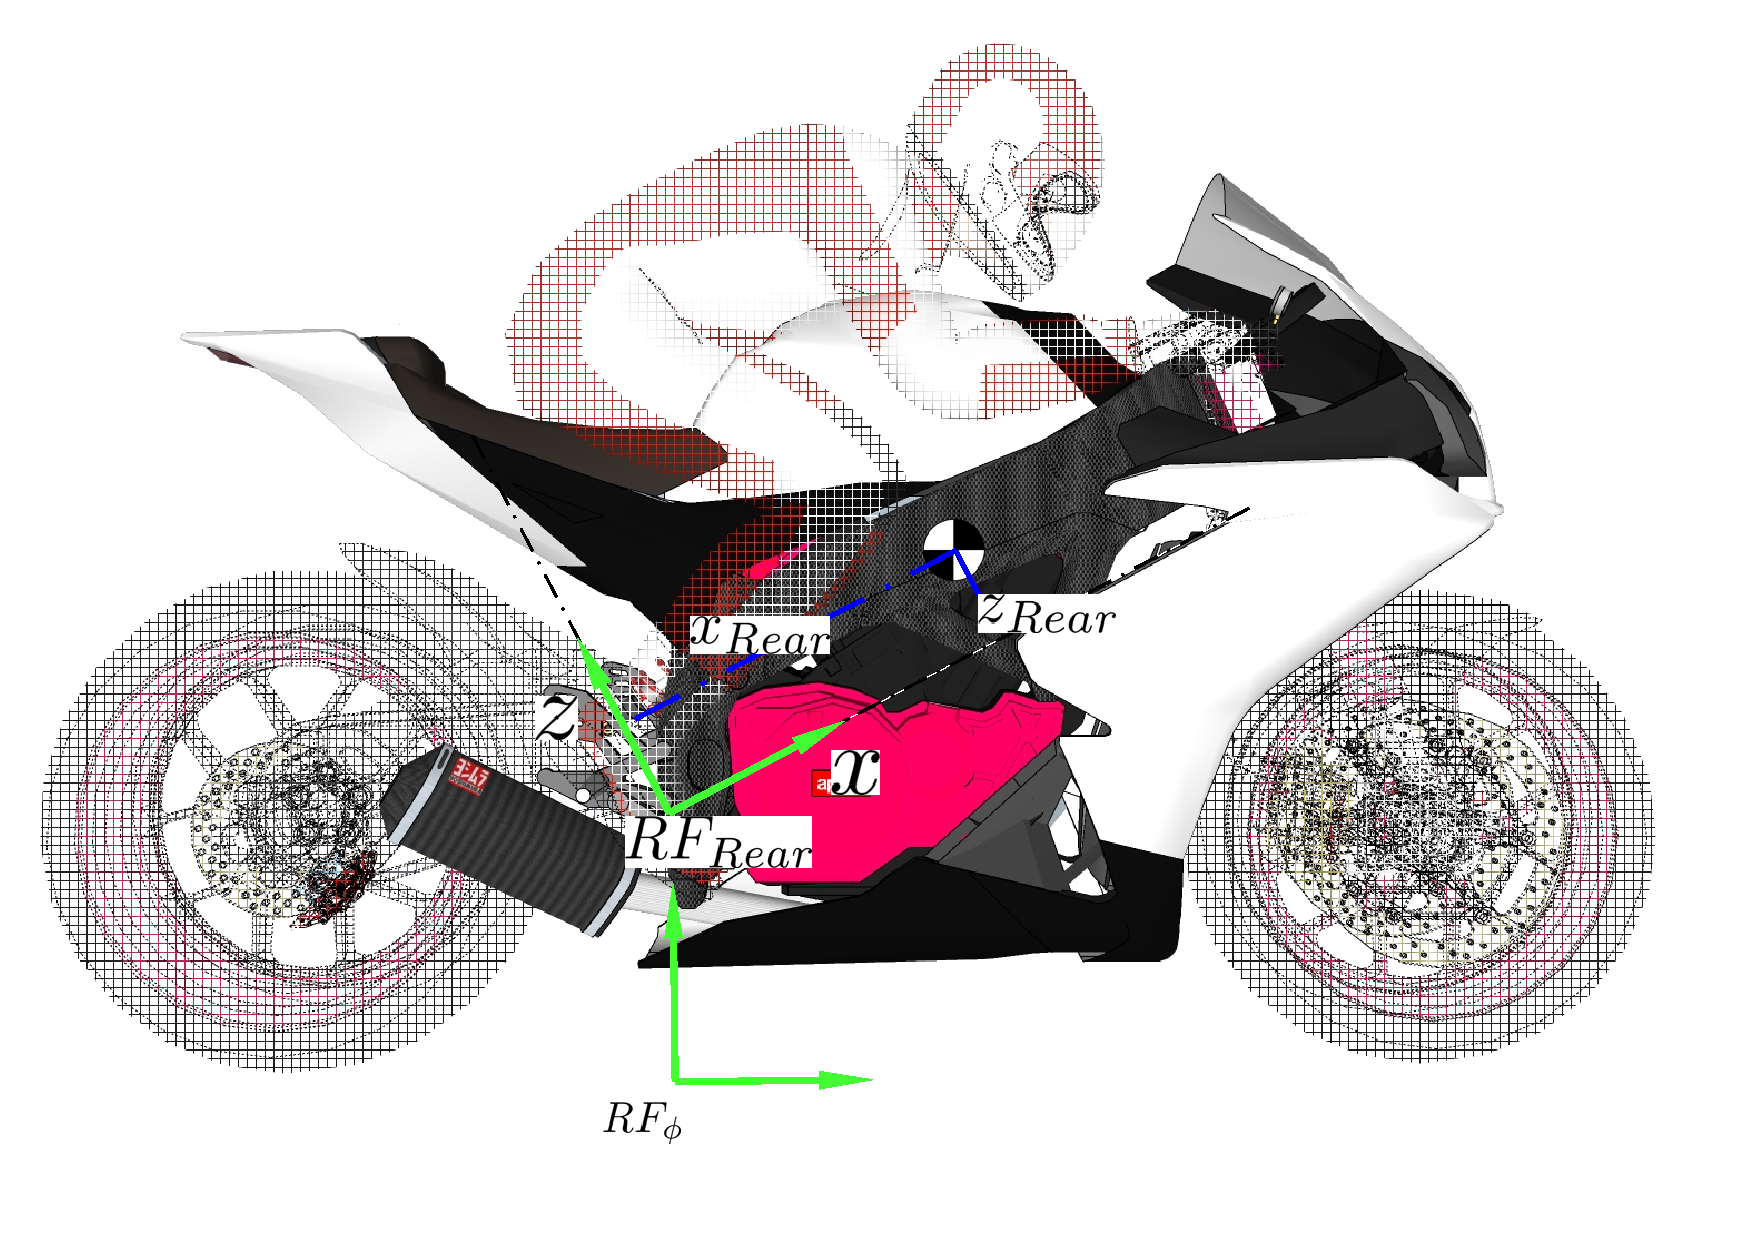
\includegraphics[width=0.5\linewidth]{Coordinates/ONLYREAR.pdf}
    \caption{CoM of the rear frame}
    \label{fig:CoMRear}
\end{figure}
%
\begin{equation}
    G_{rdr} =
    \left[
    \begin{array}{c}
        x_{rdr}\\
        0\\
        z_{rdr}
    \end{array}
    \right]
    \; \text{in} \; RF_{rear}
\end{equation}
%
\begin{figure}[h!]
    \centering
    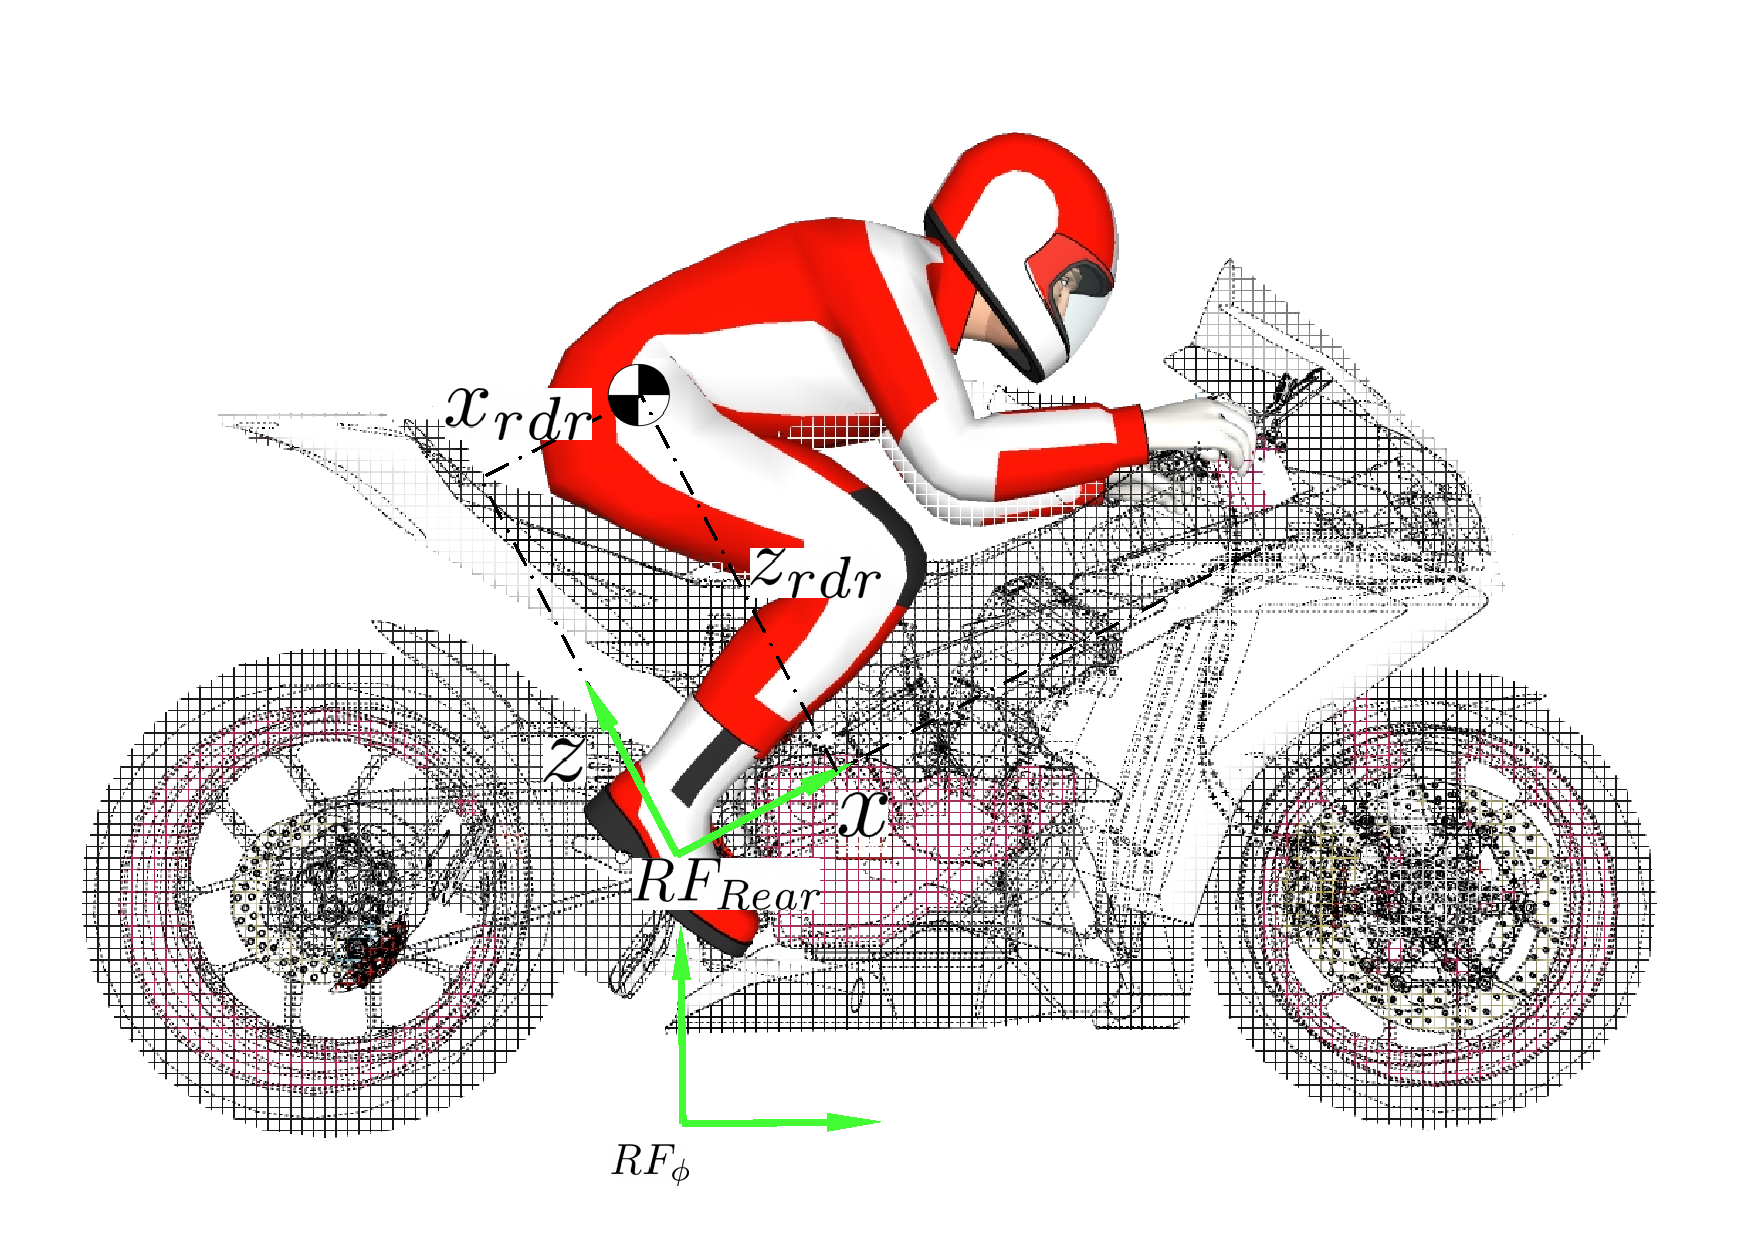
\includegraphics[width=0.5\linewidth]{Coordinates/ONLYRIDER.pdf}
    \caption{CoM of the rider}
    \label{fig:CoMrdr}
\end{figure}
%
The body representing the steering assembly is defined starting from $RF_\delta$.
%
\begin{equation}
    G_{\delta} =
    \left[
    \begin{array}{c}
        x_{\delta}\\
        0\\
        z_{\delta}
    \end{array}
    \right]
    \; \text{in} \; RF_{\delta}
\end{equation}
%
\begin{figure}[h!]
    \centering
    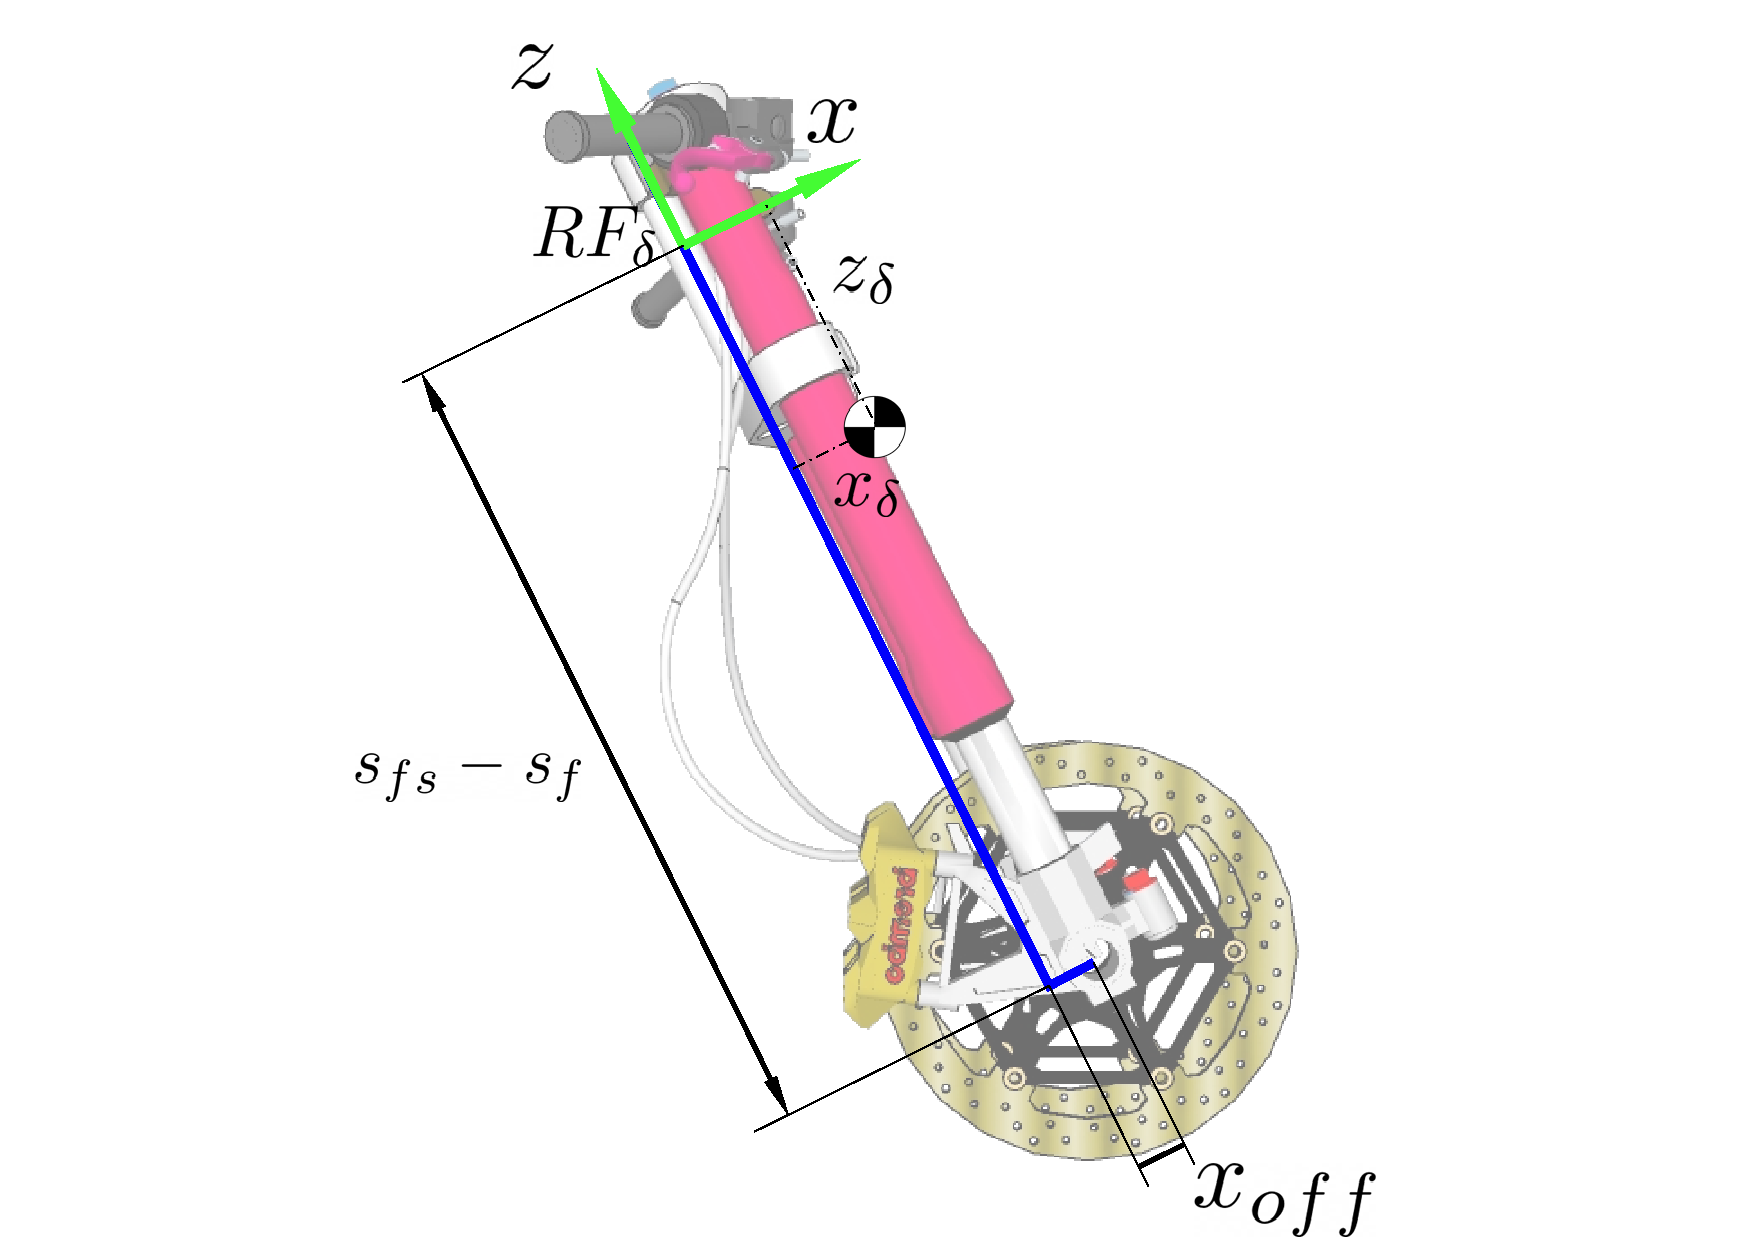
\includegraphics[width=0.6\linewidth]{Coordinates/STEER.pdf}
    \caption{CoM of the steering assembly}
    \label{fig:CoMdelta}
\end{figure}
%
where $z_{delta}$ in this case will be negative since the reference frame is define with the ISO convention.\\
The body of the swingarm in define wth the following centre of gravity starting from $RF_\eta$.
%
\begin{equation}
    G_{Swing} =
    \left[
    \begin{array}{c}
        x_{Swing}\\
        0\\
        z_{Swing}
    \end{array}
    \right]
    \; \text{in} \; RF_{\eta}
\end{equation}
%
\begin{figure}[h!]
    \centering
    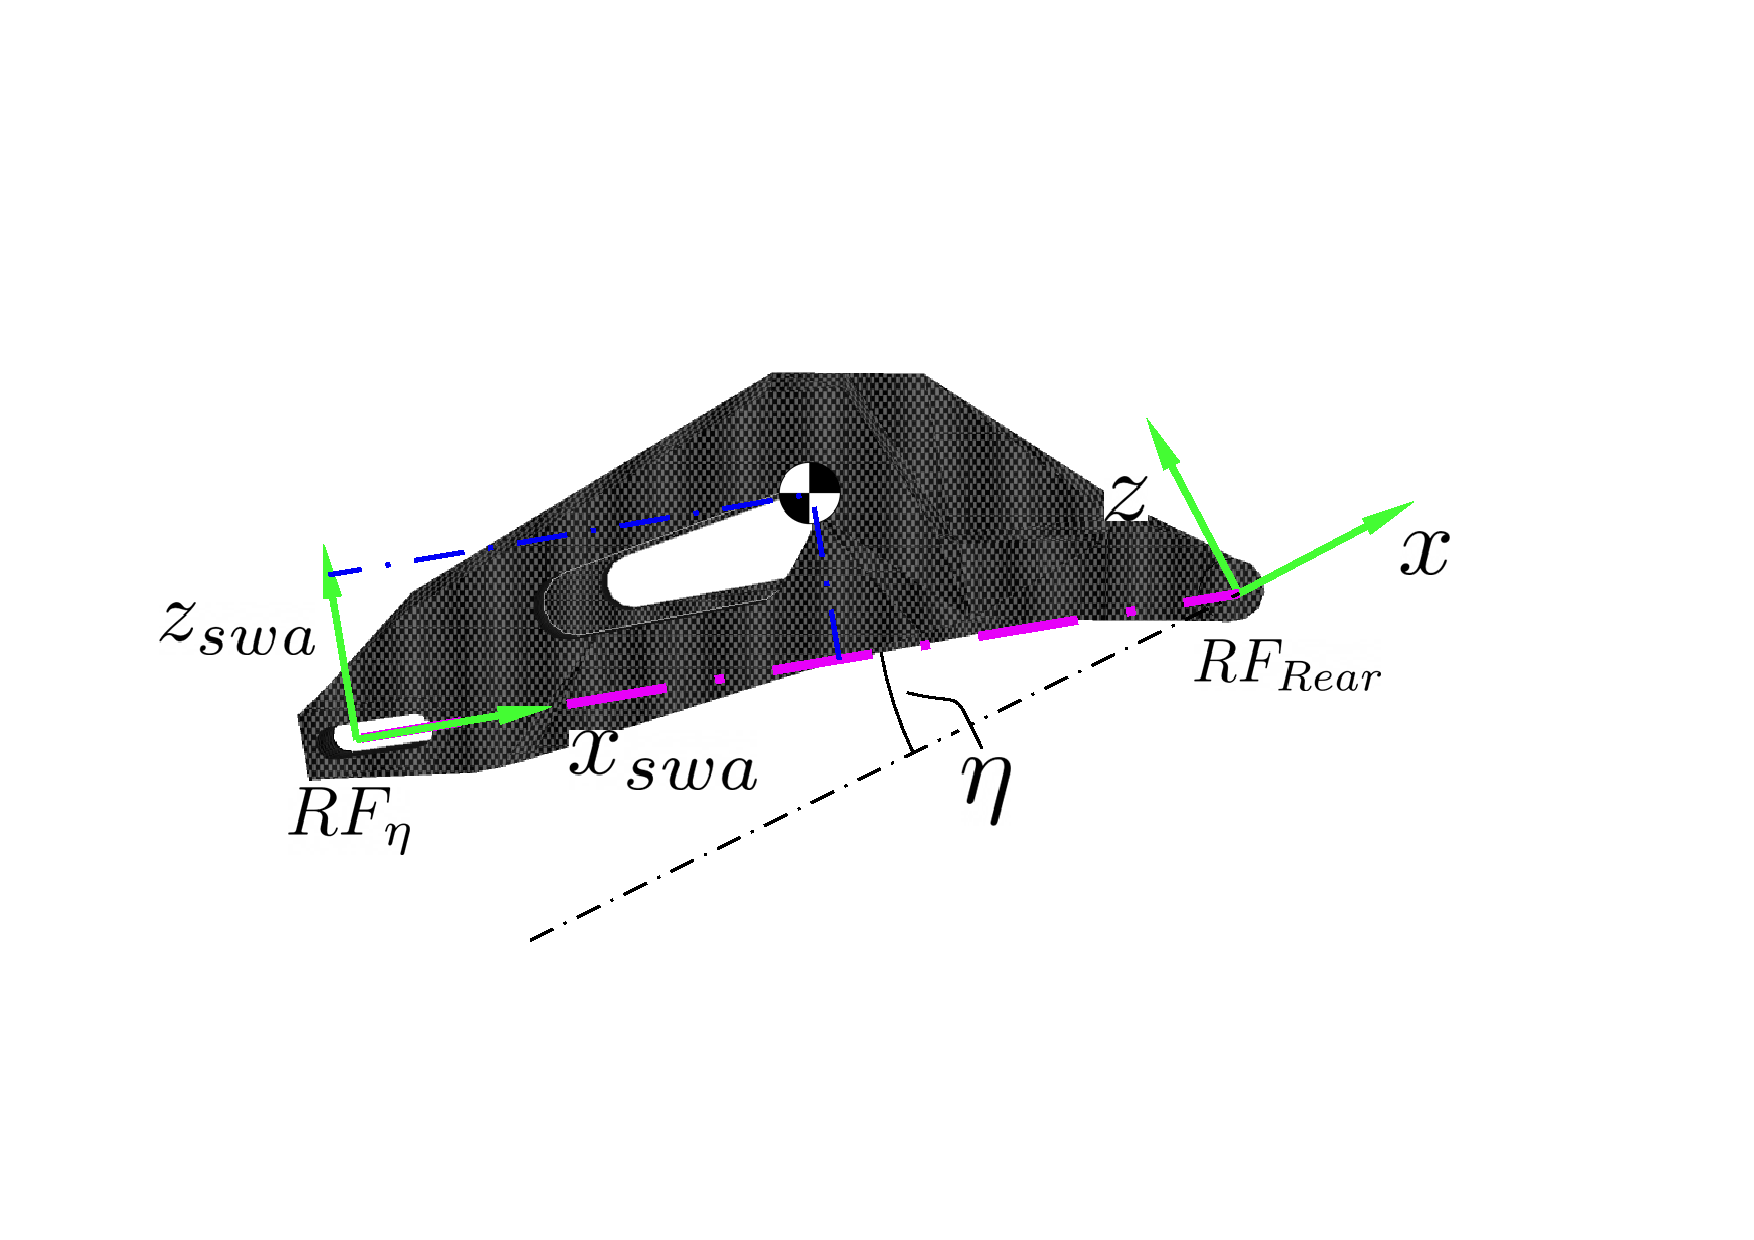
\includegraphics[width=0.6\linewidth]{Coordinates/SWINGARMONLY.pdf}
    \caption{CoM of the swingarm}
    \label{fig:CoMswa}
\end{figure}
%
The two body of the wheels have their CoM in the origin of the attached spinning reference frame.
%
\begin{equation}
    G_{FW} =
    \left[
    \begin{array}{c}
        0\\
        0\\
        0
    \end{array}
    \right]
    \; \text{in} \; RF_{FWspin}
\end{equation}
%
\begin{equation}
    G_{RW} =
    \left[
    \begin{array}{c}
        0\\
        0\\
        0
    \end{array}
    \right]
    \; \text{in} \; RF_{RWspin}
\end{equation}
%
The last body is the unsprung front suspension. However, the mass of this element is small compared to the other and it can be eventually integrated in the mass of the front wheel. The body of the unsprung suspension has as a virtual centre of mass the centre of the front wheel, wont have mass (mass$=0$) and has no inertia. This is a modelling expedient to derive the equation of motions and to transmit the reaction forces.\\
From all the previously defined centre of gravity one can define the six bodies at play with their inertial properties, mass and moment of inertia.\\
In the following sections masses and moment of inertia belonging to bodies will appear. The notation used in this thesis follow the subsequent rule. Masses and inertia are indicated with symbols $m$ and $Ix$, $Iy$, $Iz$, $Cxy$, $Cxz$, $Cyz$ in general. When addressed to a specific one a suffix is added to represent the body or the reference frame. For instance the mass of the steering assembly will be $m_\delta$.
%
\subsubsection{Centre of Mass of the motorcycle}
%
The CoM of the motorcycle can be simply computed as the weighted average sum of the masses of all the parts. This mean yields a vector of 3 components that can be projected in the rolled reference frame $RF_\phi$. Once substituted the relationship of the previous paragraph for the freezed DoF, the values of the vector are the coordinate of the CoM of the motorcycle in the rolled reference frame. 
\begin{equation}
    \label{eq:CoM}
    G_{moto} = 
    \left[ \begin{array}{c}
        XG\\
        YG\\
        ZG
    \end{array} \right]
    \text{in} \; RF_1
\end{equation}
However, the definition of $YG$ is simple and evaluated is equal to zero. This is due to the assumption that the motorcycle is always symmetric with respect to the rolled plane.
%
\subsubsection{Moment of Inertia of the motorcycle}
%
The moment of inertia of the whole motorcycle, can be computed in a similar way as the CoM.
The fist thing to derive is the angular velocity of the rolled reference frame $RF_\phi$. This will not contain angle $\theta$ because is considered as freezed.\\
The three components of the angular velocity are 
%
\begin{equation}
\label{eq:ang_vel}
\begin{array}{l} 
\displaystyle \omega_{x} \left( t \right) ={\frac {\rm d}{
{\rm d}t}}\phi \left( t \right) \\
\displaystyle \omega_{y} \left( t \right) =\Omega \left( t \right) \sin \left( \phi \left( t
 \right)  \right) \\ 
 \displaystyle \omega_{z} \left( t \right) =\Omega \left( t \right) \cos \left( \phi \left( t \right)  \right) 
\end{array} 
\end{equation}
%
Proceeding with the equation derivation the angular momentum of the whole motorcycle ic computed. The angular momentum is additive, therefore it can be calculated as the sum of all the angular momentums. Those should be calculated using as a pole the CoM of the motorcycle. The obtained vector is projected in the rolled reference frame to get rid off almost all the contribute of 
$\phi$ and evaluated considering the freezeed DoF.\\
At this point the previous relationship \ref{eq:ang_vel} can be exploited and substituted. Therefore the angular momentum can be used to generate the inertia matrix collecting $\omega_{x}$, $\omega_{y}$ and $\omega_{z}$.
%
\begin{equation}
    \mathbf{A_M} = I_{tot} 
    \left[ 
    \begin{array}{c}
        \omega_x\\
        \omega_y\\
        \omega_z
    \end{array} 
    \right]
    + \mathbf{res}
\end{equation}
%
where $I_{tot}$ is the matrix of inertia of the whole motorcycle, $\mathbf{A_M}$ is the vector of the angular momentum and $\mathbf{res}$ is the vector of residual from the matrix generation. This should be checked to be equal to zero and it is.
With the previously computed data a body can be created. This have the centre of gravity in the point of equation \ref{eq:CoM}, mass equal to the sum of all masses ($M_{tot}$) and the moment of inertia $I_{tot}$.  
%
\subsection{Dummy bodies}
\label{subsec:Dummy}
%
The moment of inertia and the masses of the different parts of the motorcycle are already inside the definition of the rigid body of the previous section. Therefore in the derivation of the equation of motion we should only consider the effect of the motion of the parts. In fact in the rigid body all the pats are frezed and considered as static. However, the dynamic component plays a great role in the motion.\\ 
One solution is to take into account only those components is to introduce a set of dummy bodies also known as anti-bodies. This bodies are defined for each moving component of the motorcycle. The dummy body has as a centre of gravity the body they are referred to, but evaluated with the internal DoF freezed. The anti-bodies, as the name suggest, has inertial properties that are the one of the real body with changed sign. This means that all dummy bodies have negative mass and negative inertia. \\
The concept of negative mass and negative inertia have no meaning in physical and real life. However, is a modelling trick to simplify the resulting equations of motion. A simple example with a double pendulum is reported in appendix \ref{app:AntiBody} to demonstrate the advantages of this method.\\
Here is reported a list of dummy bodies that have to be defined.
%
\begin{itemize}
    \setlength{\itemsep}{0pt}
    \item anti rear frame
    \item anti rider 
    \item anti steering assembly
    \item anti swingarm 
    \item anti front wheel
    \item anti rear wheel
\end{itemize}
%
There is no need to create the antibody for the unsprung front suspension since it does not have mass nor inertia. If the model consider also mass and inertia of this body then an antibody must be created to be consistent.
%
\subsection{Forces}
%
First of all the force of gravity is acting on all bodies and the acceleration of gravity is set as a vector in the negative $z$ direction due to convention choices.\\
The other external forces acting on the motorcycle are the aerodynamic drag and the force exchanged by the tyre with the ground.\\
The drag is modelled with a simple law that scale with the squared of the longitudinal velocity. It has only component in the $x$ direction in the rolled reference frame. The force act on the motorcycle rigid body.
%
\begin{equation}
    F_a = 
    \left[
    \begin{array}{c}
        -C_a u(t)^2\\
        0\\
        0
    \end{array}
    \right ]
    \text{in} \; RF_\phi
\end{equation}
%
Where $C_a$ is this case is a constant, but in theory and reality it is not. This coefficient depend on multiple thermodynamic factors and more important for this application the resisting cross section of the motorcycle and the rider. The motorcycle profile is constant, but the pilot is moving leaning forward and opening the knee at curve entrance. 
% This leads in a change up to $50\%$ in the drag coefficient. \cite{}
Moreover, the drag force has an application point which is constant in this model, but in reality change with changing configuration (position) of the driver.
%
\begin{equation}
    P_a = 
    \left[
    \begin{array}{c}
        x_a\\
        0\\
        z_a
    \end{array}
    \right ]
    \text{in} \; RF_{Rear}
\end{equation}
%
The forces of the tyre are expressed in a reference frame with the tyre itself. For the rear wheel it coincide with $RF_1$, while for the front it is necessary to rotate of an angle $\delta_f$.
The force vector on the rear wheel is composed of $Fxr(t)$ the longitudinal force, $Fyr(t)$ the lateral force and $Fzr(t)$ the vertical force.
%
\begin{equation}
    F_{RW} = 
    \left[
    \begin{array}{c}
        Fxr(t)\\
        Fyr(t)\\
        Fzr(t)
    \end{array}
    \right ]
    \text{in} \; RF_1
\end{equation}
and it is supposed as applied in the point $P_r$ and it is acting on the rear wheel. This is not true however some overturning moment will be introduced in the next section.\\
The force vector on the rear wheel is composed of $Fxf(t)$ the longitudinal force, $Fyf(t)$ the lateral force and $Fzf(t)$ the vertical force.
%
\begin{equation}
    F_{FW} = 
    \left[
    \begin{array}{c}
        Fxf(t)\\
        Fyf(t)\\
        Fzf(t)
    \end{array}
    \right ]
    \text{in} \; RF_1 \cdot R_{\delta_f}
\end{equation}
%
and it is supposed as applied in the point $P_f$ and it is acting on the front wheel. This is not true however some overturning moment will be introduced in the next section.\\
$Fxr(t)$, $Fyr(t)$, $Fxf(t)$ and $Fyf(t)$ will be defined following the Magic Formula of Pacejka\cite{pacejka2006tyre}.\\
The vertical forces are defined as a function of the penetration (equation \ref{eq:penetration}) and penetration velocity. It is modelled assuming that the tyre behave as a spring-damper (second-order) system.
%
\begin{equation}
\begin{array}{l} 
\displaystyle {\it Fzf} \left( t \right) ={\it Kp}_{f}\,p_
{f} \left( t \right) +{\it Cp}_{f}\,{\frac {\rm d}{{\rm d}t}}p_{f}
\left( t \right) \\[6pt]
\displaystyle {\it Fzr} \left( t \right) ={
\it Kp}_{r}\,p_{r} \left( t \right) +{\it Cp}_{r}\,{\frac {\rm d}{
{\rm d}t}}p_{r} \left( t \right) 
\end{array} 
\end{equation}
%
There is another force present in the model and is the one of the front suspension. It is model as a spring-damper with linear proportional and damping factor. A more complicated model can be used in future applications.
%
\begin{equation}
    F_{s} = 
    \left[
    \begin{array}{c}
        0\\
        0\\
        \displaystyle s_{f} \left( t \right) k_{{\it fs}}+ \left( {\frac {\rm d}{{\rm d}t}}s_{f} \left( t \right)  \right) c_{{\it fs}}
    \end{array}
    \right ]
    \text{in} \; RF_\delta
\end{equation}
%
For modelling purposes it is defined as acting on the origin of $RF_\delta$. However, since it is an internal force, the reacting body must be specified. In this case it is the unsprung suspension.
%
\subsection{Torques}
%
The torques acting in this dynamic model are both external and internal.
The external torques are the one acting on the wheels. Those are present for two reasons. The first is that we are considering a point of application which is not the real point of application of the forces. The contact is in fact on a patch where the distribution of forces is not known. The second reason is that the model of the magic formula \cite{pacejka2006tyre} takes into account the effect of trail and camber calculating forces and moments with respect to the point $P_r$ and $P_f$ previously defined.\\
The torques vector acting on the front wheel is:
%
\begin{equation}
    M_{RW} = 
    \left[
    \begin{array}{c}
        Mxr(t)\\
        0\\
        Mzr(t)
    \end{array}
    \right ]
    \text{in} \; RF_1
\end{equation}
%
while the momentum vector on the front wheel is:
%
\begin{equation}
    M_{FW} = 
    \left[
    \begin{array}{c}
        Mxf(t)\\
        0\\
        Mzf(t)
    \end{array}
    \right ]
    \text{in} \; RF_1 \cdot R_{\delta_f}
\end{equation}
%
Then there are other toques that are traction and braking torques. Those are acting in the $y$ direction of the reference frame attached to the wheels. Front wheel can only brake.
The traction is acting on the rear wheel and reacting on the swingarm.
%
\begin{equation}
    TB_{RW} = 
    \left[
    \begin{array}{c}
        0\\
        Myr(t)\\
        0
    \end{array}
    \right ]
    \text{in} \; RF_{RW}
\end{equation}
%
The braking torque is acting on the front wheel and reacting on the unsprung suspension.
%
\begin{equation}
    B_{FW} = 
    \left[
    \begin{array}{c}
        0\\
        Myf(t)\\
        0
    \end{array}
    \right ]
    \text{in} \; RF_{FW}
\end{equation}
%
The internal momentums are instead the torque of the steering damper, the torque applied by the rider and the torque of the rear suspension. 
The first is modelled as a viscous term.
%
\begin{equation}
    T_{d} = 
    \left[
    \begin{array}{c}
        0\\
        0\\
        -C_{\delta}\,{\frac {\rm d}{{\rm d}t}}\delta \left( t \right) 
    \end{array}
    \right ]
    \text{in} \; RF_{\delta}
\end{equation}
%
It is acting on the steering frame and reacting on the motorcycle.\\
The rider torque has only component in the $z$ direction of the $RF_\delta$.
%
\begin{equation}
    T_{r} = 
    \left[
    \begin{array}{c}
        0\\
        0\\
        \tau(t)
    \end{array}
    \right ]
    \text{in} \; RF_{\delta}
\end{equation}
%
It is acting on the steering assembly and reacting on the motorcycle rigid body.
The last internal torque is the rear suspension torque. It is actually a force of a spring-damper system applied with a certain arm. However, for modelling purposes can be written in terms of a torque with a torsional stiffness and a rotational viscosity.
%
\begin{equation}
    M_{RSusp} = 
    \left[
    \begin{array}{c}
        0\\
        \eta \left( t \right) a_{1}\,k_{{\it rs}}+ \left( {\frac {\rm d}{
            {\rm d}t}}\eta \left( t \right)  \right) a_{1}\,c_{{\it rs}} \\
        0
    \end{array}
    \right ]
    \text{in} \; RF_{Rear}
\end{equation}
%
It is acting on the swingarm and reacting on the motorcycle rigid body.
%
\begin{figure}[htb]
    \centering
    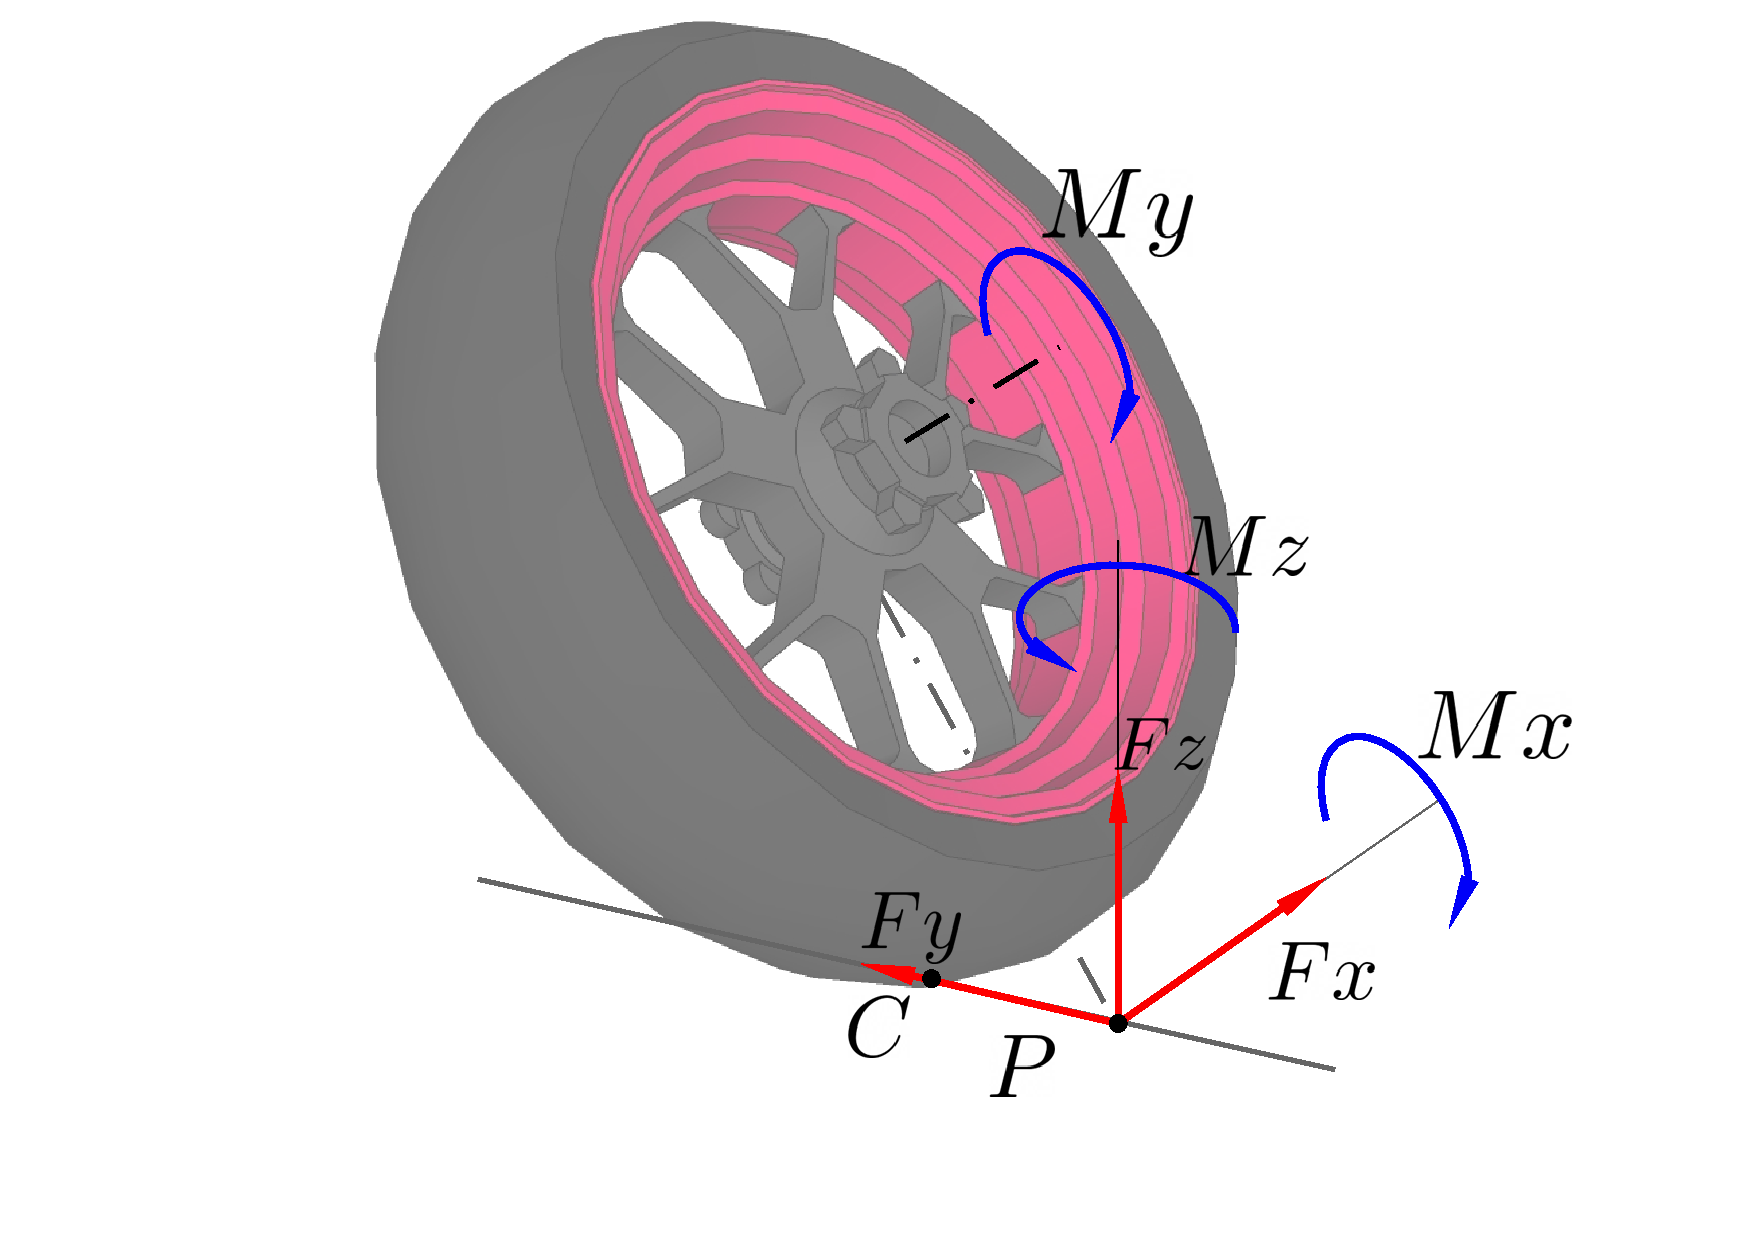
\includegraphics[width=\linewidth]{Coordinates/wheelforces.pdf}
    \caption{Forces scheme}
    \label{fig:WheelForces}
\end{figure}